\documentclass{article}
\usepackage[paper=letterpaper,margin=2cm]{geometry}
\usepackage[russian]{babel}
\usepackage[utf8]{inputenc}
\usepackage[]{graphicx}
\usepackage[usenames]{color}
\usepackage{colortbl}
\usepackage{geometry}
\usepackage{xcolor}
\usepackage{listings}
\usepackage{xlop}
\usepackage{../../lib/latex/listings-rust}

\geometry{
  a4paper,
  top=25mm, 
  right=30mm, 
  bottom=25mm, 
  left=30mm
}

\begin{document}

\begin{center}
  \section*{
    Федеральное государственное автономное образовательное учреждение\\ высшего образования\\
    «Национальный исследовательский университет ИТМО»\\
    Факультет Программной Инженерии и Компьютерной Техники \\
   }
  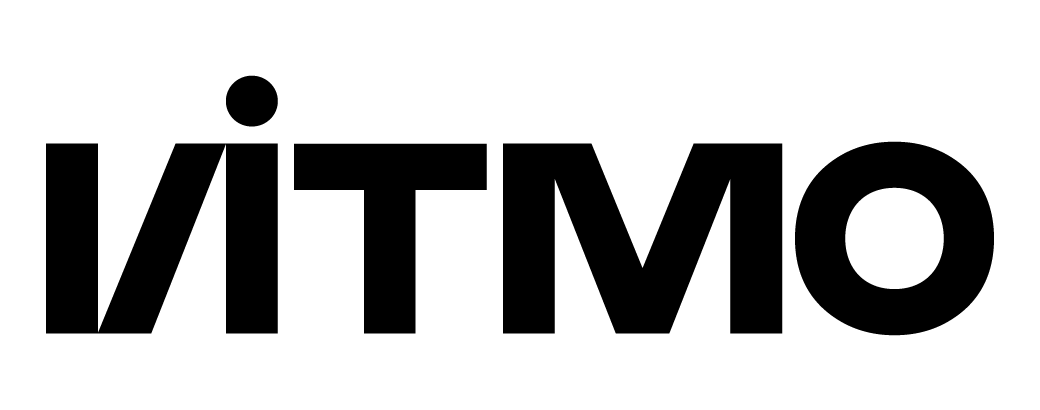
\includegraphics[scale=0.2]{../../lib/img/itmo.png}
\end{center}
\vspace{4cm}


\begin{center}
  \large \textbf{Вариант \textnumero 16}\\
  \textbf{Лабораторная работа \textnumero 2}\\
  по дисциплине\\
  \textbf{Информатика}
\end{center}

\vspace*{\fill}

\begin{flushright}
  Выполнил Студент группы P3115\\
  \textbf{Владимир Мацюк}\\
  Преподаватель: \\
  \textbf{Малышева Татьяна Алексеевна}\\
\end{flushright}

\vspace{1cm}

\begin{center}
  г. Санкт-Петербург\\
  2022г.
\end{center}

\newpage



\section*{Текст задания}


\newcommand{\A}{\cellcolor{blue!25}X}
\newcommand{\B}{\cellcolor{red!25}X}
\newcommand{\CC}{\cellcolor{green!25}X}
\newcommand{\D}{\cellcolor{cyan!25}X}

\begin{enumerate}
  \item На основании номера варианта задания выбрать набор из 4 полученных
        сообщений в виде последовательности 7-символьного кода. Построить схему декодирования классического кода Хэмминга (7;4),
        которую представить в отчёте в виде изображения. Показать, исходя из выбранных вариантов сообщений (по 4 у каждого –
        часть No1 в варианте), имеются ли в принятом сообщении ошибки, и если
        имеются, то какие. Подробно прокомментировать и записать правильное
        сообщение. \\ \textnumero 59 Message: 0010100
        $$
          \begin{tabular}{|c|c|c|c|c|c|c|c|c|}
            \hline
                    & 1     & 2     & 3     & 4     & 5     & 6     & 7     &       \\
            \hline
            Message & 0     & 0     & 1     & 0     & 1     & 0     & 0     &       \\
            \hline
            $2^x$   & $r_1$ & $r_2$ & $i_1$ & $r_3$ & $i_2$ & $i_3$ & $i_4$ & $S$   \\
            \hline
            1       & \A    &       & \A    &       & \A    &       & \A    & $s_1$ \\
            \hline
            2       &       & \B    & \B    &       &       & \B    & \B    & $s_2$ \\
            \hline
            4       &       &       &       & \CC   & \CC   & \CC   & \CC   & $s_3$ \\
            \hline
          \end{tabular}
        $$
        $$
          s_1 = r_1 \oplus i_1 \oplus i_2 \oplus i_4 = 0 \oplus 1 \oplus 1 \oplus 0 = 0
        $$$$
          s_2 = r_2 \oplus i_1 \oplus i_3 \oplus i_4 = 0 \oplus 1 \oplus 0 \oplus 0 = 1
        $$$$
          s_3 = r_3 \oplus i_2 \oplus i_3 \oplus i_4 = 0 \oplus 1 \oplus 0 \oplus 0 = 1
        $$
        \begin{center}
          Error at $Message[6]=i_3$. \\
          Corrected: 0010110
        \end{center}
  \item \textnumero 51 Message: 1010011
        $$
          \begin{tabular}{|c|c|c|c|c|c|c|c|c|}
            \hline
                    & 1     & 2     & 3     & 4     & 5     & 6     & 7     &       \\
            \hline
            Message & 1     & 0     & 1     & 0     & 0     & 1     & 1     &       \\
            \hline
            $2^x$   & $r_1$ & $r_2$ & $i_1$ & $r_3$ & $i_2$ & $i_3$ & $i_4$ & $S$   \\
            \hline
            1       & \A    &       & \A    &       & \A    &       & \A    & $s_1$ \\
            \hline
            2       &       & \B    & \B    &       &       & \B    & \B    & $s_2$ \\
            \hline
            4       &       &       &       & \CC   & \CC   & \CC   & \CC   & $s_3$ \\
            \hline
          \end{tabular}
        $$
        $$
          s_1 = r_1 \oplus i_1 \oplus i_2 \oplus i_4 = 1 \oplus 1 \oplus 0 \oplus 1 = 1
        $$$$
          s_2 = r_2 \oplus i_1 \oplus i_3 \oplus i_4 = 0 \oplus 1 \oplus 1 \oplus 1 = 1
        $$$$
          s_3 = r_3 \oplus i_2 \oplus i_3 \oplus i_4 = 0 \oplus 0 \oplus 1 \oplus 1 = 0
        $$
        \begin{center}
          Error at $Message[3]=i_1$. \\
          Corrected: 1010101
        \end{center}
  \item \textnumero 73 Message: 1000011
        $$
          \begin{tabular}{|c|c|c|c|c|c|c|c|c|}
            \hline
                    & 1     & 2     & 3     & 4     & 5     & 6     & 7     &       \\
            \hline
            Message & 0     & 0     & 1     & 0     & 1     & 0     & 1     &       \\
            \hline
            $2^x$   & $r_1$ & $r_2$ & $i_1$ & $r_3$ & $i_2$ & $i_3$ & $i_4$ & $S$   \\
            \hline
            1       & \A    &       & \A    &       & \A    &       & \A    & $s_1$ \\
            \hline
            2       &       & \B    & \B    &       &       & \B    & \B    & $s_2$ \\
            \hline
            4       &       &       &       & \CC   & \CC   & \CC   & \CC   & $s_3$ \\
            \hline
          \end{tabular}
        $$
        $$
          s_1 = r_1 \oplus i_1 \oplus i_2 \oplus i_4 = 0 \oplus 1 \oplus 1 \oplus 1 = 1
        $$$$
          s_2 = r_2 \oplus i_1 \oplus i_3 \oplus i_4 = 0 \oplus 1 \oplus 0 \oplus 1 = 0
        $$$$
          s_3 = r_3 \oplus i_2 \oplus i_3 \oplus i_4 = 0 \oplus 1 \oplus 0 \oplus 1 = 0
        $$
        \begin{center}
          Error at $Message[1]=r_1$. \\
          Corrected: 1010101
        \end{center}
  \item \textnumero 95 Message: 1011110
        $$
          \begin{tabular}{|c|c|c|c|c|c|c|c|c|}
            \hline
                    & 1     & 2     & 3     & 4     & 5     & 6     & 7     &       \\
            \hline
            Message & 1     & 0     & 1     & 1     & 1     & 1     & 0     &       \\
            \hline
            $2^x$   & $r_1$ & $r_2$ & $i_1$ & $r_3$ & $i_2$ & $i_3$ & $i_4$ & $S$   \\
            \hline
            1       & \A    &       & \A    &       & \A    &       & \A    & $s_1$ \\
            \hline
            2       &       & \B    & \B    &       &       & \B    & \B    & $s_2$ \\
            \hline
            4       &       &       &       & \CC   & \CC   & \CC   & \CC   & $s_3$ \\
            \hline
          \end{tabular}
        $$
        $$
          s_1 = r_1 \oplus i_1 \oplus i_2 \oplus i_4 = 1 \oplus 1 \oplus 1 \oplus 0 = 1
        $$$$
          s_2 = r_2 \oplus i_1 \oplus i_3 \oplus i_4 = 0 \oplus 1 \oplus 1 \oplus 0 = 0
        $$$$
          s_3 = r_3 \oplus i_2 \oplus i_3 \oplus i_4 = 1 \oplus 1 \oplus 1 \oplus 0 = 1
        $$
        \begin{center}
          Error at $Message[5]=i_2$. \\
          Corrected: 1011010
        \end{center}
  \item На основании номера варианта задания выбрать 1 полученное сообщение в
        виде последовательности 11-символьного кода. Построить схему декодирования классического кода Хэмминга (15;11),
        которую представить в отчёте в виде изображения. Показать, исходя из выбранного варианта сообщений (по 1 у каждого –
        часть No2 в варианте), имеются ли в принятом сообщении ошибки, и если
        имеются, то какие. Подробно прокомментировать и записать правильное
        сообщение. \\
        \textnumero 17 Message: 011000100010001
        $$
          \begin{tabular}{|c|c|c|c|c|c|c|c|c|c|c|c|c|c|c|c|c|}
            \hline
                    & 1     & 2     & 3     & 4     & 5     & 6     & 7     & 8     & 9     & 10    & 11    & 12    & 13    & 14       & 15       &       \\
            \hline
            Message & 0     & 1     & 1     & 0     & 0     & 0     & 1     & 0     & 0     & 0     & 1     & 0     & 0     & 0        & 1        &       \\
            \hline
            $2^x$   & $r_1$ & $r_2$ & $i_1$ & $r_3$ & $i_2$ & $i_3$ & $i_4$ & $r_4$ & $i_5$ & $i_6$ & $i_7$ & $i_8$ & $i_9$ & $i_{10}$ & $i_{11}$ & $S$   \\
            \hline
            1       & \A    &       & \A    &       & \A    &       & \A    &       & \A    &       & \A    &       & \A    &          & \A       & $s_1$ \\
            \hline
            2       &       & \B    & \B    &       &       & \B    & \B    &       &       & \B    & \B    &       &       & \B       & \B       & $s_2$ \\
            \hline
            4       &       &       &       & \CC   & \CC   & \CC   & \CC   &       &       &       &       & \CC   & \CC   & \CC      & \CC      & $s_3$ \\
            \hline
            8       &       &       &       &       &       &       &       & \D    & \D    & \D    & \D    & \D    & \D    & \D       & \D       & $s_4$ \\
            \hline
          \end{tabular}
        $$
        $$
          s_1 = r_1 \oplus i_1 \oplus i_2 \oplus i_4 \oplus i_5 \oplus i_7 \oplus i_9 \oplus i_{11}= 0 \oplus 1 \oplus0 \oplus1 \oplus0 \oplus1 \oplus0 \oplus1 = 0
        $$$$
          s_2 = r_2 \oplus i_1 \oplus i_3 \oplus i_4 \oplus i_6 \oplus i_7 \oplus i_{10} \oplus i_{11} =1  \oplus1 \oplus0 \oplus1 \oplus0 \oplus1 \oplus0 \oplus1 = 1
        $$$$
          s_3 = r_3 \oplus i_2 \oplus i_3 \oplus i_4 \oplus i_8 \oplus i_9 \oplus i_{10} \oplus i_{11} =  0 \oplus0 \oplus0 \oplus1 \oplus0 \oplus0 \oplus0 \oplus1 = 0
        $$
        $$
          s_3 = r_4 \oplus i_5 \oplus i_6 \oplus i_7 \oplus i_8 \oplus i_9 \oplus i_{10} \oplus i_{11} = 0\oplus0\oplus0\oplus1\oplus0\oplus0\oplus0\oplus1 = 0
        $$
        \begin{center}
          Error at $Message[2]=r_2$.\\
          Corrected: 001000100010001
        \end{center}
  \item  Сложить номера всех 5 вариантов заданий. Умножить полученное число
        на 4. Принять данное число как число информационных разрядов в
        передаваемом сообщении. Вычислить для данного числа минимальное
        число проверочных разрядов и коэффициент избыточности. $$ m = (59 + 51 + 73 + 95 + 17) \cdot 4 = 1180 $$
        $$ \left. \begin{array}{rr}
            m = 1180 \\
            r \geq \log_2(r+m+1)
          \end{array} \right\} \Rightarrow r = 11$$
        $$\frac{11}{11+1180} \approx 0.00923$$
  \item Написать программу на любом языке программирования,
        которая на вход из командной строки получает набор из 7 цифр «0» и «1»,
        записанных подряд, анализирует это сообщение на основе классического
        кода Хэмминга (7,4), а затем выдает правильное сообщение (только
        информационные биты) и указывает бит с ошибкой при его наличии. \lstset{
          inputencoding=utf8,
          frame=single,
          language=Rust,
          breaklines=true,
          numbers=left,
          postbreak=\mbox{\textcolor{red}{$\hookrightarrow$}\space},
          extendedchars=false,
          showspaces=false,
          showstringspaces=false,
          basicstyle=\footnotesize\ttfamily,
          identifierstyle=\bf\ttfamily\color[HTML]{2a72de},
          commentstyle=\color[rgb]{0.133,0.545,0.133},
          stringstyle=\color[rgb]{0.133,0.545,0.133},
          keywordstyle=\color[HTML]{5804cf}
        }
        \lstinputlisting{./hamming/src/main.rs}
\end{enumerate}


\section*{Вывод}
Тут потом будет вывод.
\end{document}
